% !TeX program = xelatex
\documentclass[a4paper,12pt]{article}

% ===== 1. KHỔ GIẤY, LỀ TRANG, FONT =====
\usepackage[left=3cm,right=2cm,top=2cm,bottom=2cm,footskip=1cm]{geometry}
\usepackage{fontspec}

\IfFontExistsTF{Times New Roman}{
  \setmainfont{Times New Roman}
}{
  \IfFileExists{fonts/times.ttf}{
    \setmainfont{times.ttf}[
      Path=fonts/,
      BoldFont=timesbd.ttf,
      ItalicFont=timesi.ttf,
      BoldItalicFont=timesbi.ttf]
  }{
    \IfFontExistsTF{TeX Gyre Termes}{
      \setmainfont{TeX Gyre Termes}
      \PackageWarningNoLine{MauBaoCao}{Times New Roman unavailable; using TeX Gyre Termes}
    }{
      \setmainfont{DejaVu Serif}
      \PackageWarningNoLine{MauBaoCao}{Times New Roman unavailable; using DejaVu Serif}
    }
  }
}
\usepackage{indentfirst}
\usepackage{microtype}
\usepackage{graphicx}
\usepackage{float}
\usepackage{tikz}
\usepackage{array,tabularx,booktabs,longtable}
\usepackage{enumitem}
\usepackage{titlesec}
\usepackage{tocloft}
\usepackage{caption}
\usepackage{xurl}
\usepackage[unicode,hidelinks]{hyperref}
\urlstyle{same}

\renewcommand{\normalsize}{\fontsize{13}{19.5}\selectfont}
\AtBeginDocument{\normalsize}
\setlength{\parindent}{0.5cm}
\setlength{\parskip}{4pt}
\setlength{\emergencystretch}{2em}
\raggedbottom
\setlist{topsep=4pt,itemsep=2pt,parsep=0pt,leftmargin=*}

% ===== 2. BA CẤP TIÊU ĐỀ: 1 / 1.1 / 1.1.1 =====
\setcounter{secnumdepth}{3}
\setcounter{tocdepth}{3}
\renewcommand{\thesection}{\arabic{section}}
\renewcommand{\thesubsection}{\thesection.\arabic{subsection}}
\renewcommand{\thesubsubsection}{\thesubsection.\arabic{subsubsection}}
\titleformat{\section}[hang]
  {\normalfont\fontsize{16}{20}\selectfont\bfseries}
  {\thesection.}{0.6em}{}
\titleformat{\subsection}[hang]
  {\normalfont\fontsize{14}{18}\selectfont\bfseries}
  {\thesubsection}{0.6em}{}
\titleformat{\subsubsection}[hang]
  {\normalfont\fontsize{13}{17}\selectfont\bfseries}
  {\thesubsubsection}{0.6em}{}
\titlespacing*{\section}{0pt}{16pt}{8pt}
\titlespacing*{\subsection}{0pt}{12pt}{6pt}
\titlespacing*{\subsubsection}{0pt}{8pt}{4pt}

% ===== 3. MỤC LỤC VÀ SỐ TRANG =====
\renewcommand{\contentsname}{MỤC LỤC}
\renewcommand{\refname}{Tài liệu tham khảo}
\renewcommand{\cfttoctitlefont}{\fontsize{16}{20}\selectfont\bfseries}
\setlength{\cftbeforetoctitleskip}{0pt}
\setlength{\cftaftertoctitleskip}{18pt}
\renewcommand{\cftsecfont}{\normalfont\bfseries}
\renewcommand{\cftsecpagefont}{\normalfont\bfseries}
\renewcommand{\cftsubsecfont}{\normalfont}
\renewcommand{\cftsubsubsecfont}{\normalfont}
\renewcommand{\cftsecleader}{\cftdotfill{\cftdotsep}}
\cftsetindents{section}{0em}{2em}
\cftsetindents{subsection}{2em}{3em}
\cftsetindents{subsubsection}{5em}{4em}
\setlength{\cftbeforesecskip}{6pt}
\makeatletter
\def\ps@plain{%
  \let\@oddhead\@empty\let\@evenhead\@empty
  \def\@oddfoot{\hfil{\normalfont\fontsize{11}{13}\selectfont\thepage}\hfil}%
  \let\@evenfoot\@oddfoot}
\makeatother
\pagestyle{plain}

% ===== 4. BẢNG, HÌNH, CHÚ THÍCH =====
\renewcommand{\tablename}{Bảng}
\renewcommand{\figurename}{Hình}
\DeclareCaptionFont{reportcaption}{\fontsize{12}{15}\selectfont}
\captionsetup{font=reportcaption,labelfont=bf,labelsep=period,
  justification=centering,skip=6pt}
\newcolumntype{Y}{>{\raggedright\arraybackslash}X}
\newcommand{\bangfont}{\fontsize{12}{15}\selectfont}

% ===== 5. THÔNG TIN TRANG BÌA =====
\newcommand{\DonViChuQuan}{ĐẠI HỌC QUỐC GIA HÀ NỘI}
\newcommand{\TenTruong}{TRƯỜNG ĐẠI HỌC CÔNG NGHỆ}
\newcommand{\LoaiBaoCao}{BÁO CÁO TIẾN ĐỘ DỰ ÁN 1}
\newcommand{\TenMonHoc}{ĐIỆN TOÁN ĐÁM MÂY}
\newcommand{\TenDeTai}{SatiBot -- Quản lý và tương tác với các tài nguyên AWS bằng ngôn ngữ tự nhiên}
\newcommand{\GiangVien}{TS. Hoàng Xuân Tùng}
\newcommand{\SoNhom}{Nhóm 10}
\newcommand{\LopMonHoc}{INT3319 1}
\newcommand{\DiaDiemThoiGian}{Hà Nội, Tháng 10/2026}
\hypersetup{pdftitle={BÁO CÁO TIẾN ĐỘ DỰ ÁN 1 - SATIBOT},pdfauthor={Nhóm 10}}

\begin{document}

% ===== 6. TRANG BÌA =====
\begin{titlepage}
\thispagestyle{empty}
\begin{tikzpicture}[remember picture,overlay]
  \draw[line width=2pt]
    ([xshift=3cm,yshift=-2cm]current page.north west)
    rectangle ([xshift=-2cm,yshift=2cm]current page.south east);
  \draw[line width=0.5pt]
    ([xshift=3.12cm,yshift=-2.12cm]current page.north west)
    rectangle ([xshift=-2.12cm,yshift=2.12cm]current page.south east);
\end{tikzpicture}\par
\centering
\setlength{\parindent}{0pt}
\setlength{\parskip}{0pt}
\vspace*{0.8cm}
{\fontsize{14}{18}\selectfont\bfseries\DonViChuQuan\par}
\vspace{0.15cm}
{\fontsize{15}{20}\selectfont\bfseries\TenTruong\par}
\vspace{0.25cm}
\rule{5cm}{0.4pt}\par
\vspace{0.5cm}

\IfFileExists{Image/logo.png}{
  
\includegraphics[width=3.8cm,height=3.8cm,keepaspectratio]{Image/logo.png}
}{
  \fbox{\parbox[c][3.4cm][c]{3.4cm}{\centering
    \fontsize{11}{14}\selectfont LOGO TRƯỜNG}}
}\par
\vspace{0.7cm}
{\fontsize{22}{27}\selectfont\bfseries\LoaiBaoCao\par}
\vspace{0.35cm}
\begin{minipage}{0.9\textwidth}\centering
  {\fontsize{15}{20}\selectfont\bfseries MÔN HỌC: \TenMonHoc\par}
\end{minipage}\par
\vspace{0.6cm}
{\fontsize{13}{17}\selectfont\bfseries ĐỀ TÀI\par}
\vspace{0.12cm}
\begin{minipage}{0.9\textwidth}\centering
  {\fontsize{16}{21}\selectfont\bfseries\TenDeTai\par}
\end{minipage}\par
\vspace{0.65cm}
{\fontsize{13}{19.5}\selectfont
\renewcommand{\arraystretch}{1.1}
\begin{tabular}{@{}>{\raggedright\arraybackslash\bfseries}p{5.2cm}>{\raggedright\arraybackslash}p{8cm}@{}}
  Giảng viên hướng dẫn: & \GiangVien\\
  Nhóm thực hiện: & \SoNhom\\
  Sinh viên thực hiện: & Cao Anh Minh \textbf{(Trưởng nhóm)}\\
                      & Trịnh Thiên Quang\\
                      & Phạm Đức Hùng\\
                      & Nguyễn Đức Huy\\
  Lớp môn học: &  \LopMonHoc
\end{tabular}\par}
\vfill
{\fontsize{13}{17}\selectfont\bfseries\DiaDiemThoiGian\par}
\vspace*{0.5cm}
\end{titlepage}

% ===== 7. MỤC LỤC TỰ ĐỘNG =====
\pagenumbering{roman}
\tableofcontents
\clearpage
\pagenumbering{arabic}

% ===== 8. NỘI DUNG BÁO CÁO =====

\section{TỔNG QUAN VỀ DỰ ÁN}

\subsection{Giới thiệu chung về tính năng dự án}

Hiện nay, Amazon Web Services (AWS) là một trong những nền tảng điện toán đám mây phổ biến nhất phục vụ học tập, nghiên cứu và triển khai ứng dụng. Tuy nhiên, việc khởi tạo và quản trị tài nguyên thông qua giao diện web (AWS Management Console) đòi hỏi nhiều thao tác thủ công, điều hướng qua nhiều màn hình cấu hình phức tạp và rất dễ nhầm lẫn. Trong khi đó, việc sử dụng giao diện dòng lệnh (AWS CLI) hoặc viết tập lệnh tự động lại yêu cầu ghi nhớ chính xác cú pháp câu lệnh, cấu trúc tệp cấu hình JSON và các tham số kỹ thuật. Đối với sinh viên, lập trình viên mới tiếp cận điện toán đám mây hoặc người quản lý kỹ thuật, các rào cản này làm chậm quá trình vận hành, đồng thời tiềm ẩn nguy cơ cấu hình sai gây mất an toàn thông tin hoặc phát sinh chi phí ngoài ý muốn.

Nhằm giải quyết vấn đề trên, nhóm thực hiện đề tài xây dựng SatiBot -- ứng dụng ChatOps hỗ trợ quản lý, cấu hình và giám sát tài nguyên AWS thông qua câu lệnh bằng ngôn ngữ tự nhiên tiếng Việt. Bằng cách kết hợp mô hình ngôn ngữ lớn (LLM) hỗ trợ cơ chế \textit{Function Calling} với thư viện AWS SDK (Boto3), SatiBot hoạt động như một trợ lý hỗ trợ thao tác hạ tầng. Người dùng chỉ cần gửi yêu cầu bằng tiếng Việt qua giao diện chat; hệ thống sẽ phân tích ý định, kiểm tra tính hợp lệ và độ an toàn của câu lệnh, sau đó gọi các API tương ứng của AWS và trả về kết quả thực thi kèm theo thông tin chi tiết, cảnh báo rủi ro hoặc hướng dẫn xử lý tiếp theo.

\subsection{Giới thiệu người dùng của dự án}

Hệ thống SatiBot hướng tới 03 nhóm người dùng chính với nhu cầu sử dụng thực tế như sau:

\begin{itemize}
  \item \textbf{Lập trình viên và kỹ sư vận hành (Developers / DevOps Engineers):} Cần khởi tạo nhanh môi trường thử nghiệm, cấu hình máy chủ, cập nhật mã nguồn hàm serverless hoặc xem log hệ thống trong quá trình phát triển ứng dụng. SatiBot giúp nhóm này thực hiện các tác vụ lặp đi lặp lại nhanh hơn ngay trên khung chat mà không cần chuyển đổi qua lại giữa nhiều trang trên AWS Console.
  \item \textbf{Sinh viên ngành Công nghệ thông tin / Điện toán đám mây:} Cần môi trường thực hành trực quan cho các môn học về mạng và hạ tầng đám mây. Hệ thống cung cấp cơ chế kiểm tra an toàn (guardrails), giúp sinh viên tránh các lỗi phổ biến như mở cổng mạng công khai nguy hiểm, quên tắt máy ảo hoặc chọn nhầm các gói cấu hình vượt quá phạm vi gói miễn phí (AWS Free Tier).
  \item \textbf{Quản lý kỹ thuật và chủ dự án (Tech Leads / Project Managers):} Cần theo dõi nhanh tình trạng hoạt động của tài nguyên, kiểm tra phân quyền (IAM Audit) và kiểm soát chi phí sử dụng hàng tháng (FinOps) bằng ngôn ngữ tự nhiên mà không cần thành thạo cú pháp dòng lệnh AWS CLI.
\end{itemize}

\subsection{Cách thức và quy trình người dùng sử dụng sản phẩm để đạt mục đích}

Để đáp ứng nhu cầu quản trị hạ tầng cơ bản, SatiBot hỗ trợ 04 dịch vụ chính của AWS gồm: Amazon EC2, Amazon S3, AWS IAM và AWS Lambda. Để mô tả tổng quan cách người dùng tương tác với hệ thống, mối quan hệ giữa 03 nhóm tác nhân (Lập trình viên, Sinh viên, Quản lý) và các ca sử dụng chức năng được thể hiện trong Sơ đồ Use Case tổng thể (Hình~\ref{fig:usecase}).

\begin{figure}[H]
\centering
\fbox{\parbox[c][7cm][c]{0.88\textwidth}{\centering 
  \vspace{0.4cm}
  {\fontsize{13}{16}\selectfont\bfseries SƠ ĐỒ USE CASE TỔNG THỂ HỆ THỐNG SATIBOT}\\[0.4cm]
  \parbox{0.78\textwidth}{\centering\small\itshape
  }
  \vspace{0.4cm}
}}
\caption{Sơ đồ Use Case tổng thể mô tả các ca sử dụng của hệ thống SatiBot}
\label{fig:usecase}
\end{figure}

Dưới đây là chi tiết về mục đích và quy trình tương tác thực tế của người dùng đối với từng nhóm tính năng của 04 dịch vụ AWS nòng cốt.

\subsubsection{Nhóm kịch bản và quy trình quản trị Amazon EC2}

Dịch vụ máy chủ ảo (Amazon Elastic Compute Cloud - EC2) là hạ tầng phục vụ việc triển khai và chạy ứng dụng. SatiBot hỗ trợ 05 quy trình quản lý trạng thái và cấu hình máy ảo như sau:

\begin{enumerate}
  \item \textbf{Khởi tạo máy chủ chuẩn hóa và xử lý trùng lặp tên:}
  \begin{itemize}
    \item \textit{Mục đích:} Tạo nhanh máy ảo để thử nghiệm hoặc triển khai website mà không phải cấu hình thủ công nhiều bước, đồng thời xử lý trường hợp tên máy bị trùng.
    \item \textit{Quy trình người dùng:} 
    \begin{itemize}
      \item Nhắn yêu cầu tạo máy kèm mục đích sử dụng (ví dụ: "Tạo cho tôi một máy chủ Ubuntu để chạy web demo, mở cổng SSH và HTTP").
      \item Nếu tên máy đã tồn tại, hệ thống đưa ra 3 lựa chọn: tiếp tục sử dụng máy cũ, đổi tên máy mới hoặc xóa máy cũ để tạo lại.
      \item Nhận kết quả thành công gồm: Địa chỉ IP máy chủ, link tải file khóa SSH (.pem) và câu lệnh kết nối mẫu.
    \end{itemize}
  \end{itemize}

  \item \textbf{Kiểm soát chi phí và xử lý vượt hạn mức tài nguyên (Cost Guardrails \& Quota):}
  \begin{itemize}
    \item \textit{Mục đích:} Tránh việc chọn nhầm máy cấu hình cao gây phát sinh chi phí lớn, đồng thời hướng dẫn cách xử lý khi tài khoản chạm ngưỡng hạn mức tạo máy ảo (vCPU quota).
    \item \textit{Quy trình người dùng:}
    \begin{itemize}
      \item Nhắn yêu cầu loại máy mong muốn (ví dụ: \textit{''Tạo máy ảo c5.4xlarge 16 vCPU''} hoặc \textit{''Tạo thêm 1 máy ảo Ubuntu''}).
      \item Xem phản hồi từ hệ thống:
      \begin{itemize}
        \item \textit{Nếu yêu cầu máy cấu hình cao, chi phí lớn:} Hệ thống cảnh báo chi phí ước tính hàng tháng, tạm dừng thao tác và yêu cầu người dùng xác nhận nếu vẫn muốn tiếp tục khởi tạo.
        \item \textit{Nếu tài khoản chạm giới hạn vCPU:} Hệ thống giải thích nguyên nhân và liệt kê danh sách các máy ảo đang chạy để người dùng cân nhắc tắt bớt máy không dùng.
      \end{itemize}
      \item Người dùng chọn phương án: chuyển về gói miễn phí (Free Tier), tắt bớt máy cũ hoặc gửi yêu cầu nâng hạn mức lên AWS.
    \end{itemize}
  \end{itemize}

  \item \textbf{Tra cứu và điều khiển vòng đời máy chủ (Bật / Tắt / Khởi động lại / Xóa):}
  \begin{itemize}
    \item \textit{Mục đích:} Theo dõi danh sách máy ảo và điều khiển trạng thái bật/tắt kịp thời nhằm tránh lãng phí tài nguyên và kiểm soát chi phí vận hành.
    \item \textit{Quy trình người dùng:}
    \begin{itemize}
      \item Nhắn câu lệnh tra cứu hoặc điều khiển (ví dụ: \textit{''Liệt kê các máy ảo đang chạy''}, \textit{''Tắt máy ảo web-demo''}, \textit{''Khởi động lại máy i-0abc123''}, \textit{''Xóa máy ảo staging''}).
      \item Xem bảng thông tin gồm ID, tên máy, trạng thái, IP công khai và thời gian chạy; nhận thông báo trạng thái cập nhật (kèm IP mới khi bật lại máy).
      \item Với thao tác xóa: Hệ thống cảnh báo mất dữ liệu và yêu cầu người dùng gõ xác nhận trước khi thực hiện xóa máy.
    \end{itemize}
  \end{itemize}

  \item \textbf{Giám sát hiệu năng và phát hiện máy chủ lãng phí (FinOps \& CloudWatch):}
  \begin{itemize}
    \item \textit{Mục đích:} Theo dõi mức độ sử dụng tài nguyên để tắt các máy nhàn rỗi nhằm tiết kiệm chi phí, hoặc nhận biết máy bị quá tải để kịp thời nâng cấp.
    \item \textit{Quy trình người dùng:}
    \begin{itemize}
      \item Nhắn câu hỏi kiểm tra (ví dụ: \textit{''Kiểm tra CPU máy i-0abc123 trong 24 giờ qua''}).
      \item Nhận số liệu đánh giá chi tiết:
      \begin{itemize}
        \item \textit{Cảnh báo lãng phí:} Nếu máy chạy không tải kéo dài, hệ thống đưa ra gợi ý tắt máy để tiết kiệm chi phí.
        \item \textit{Cảnh báo nghẽn tải:} Nếu mức sử dụng CPU liên tục ở mức cao, hệ thống cảnh báo quá tải và gợi ý nâng cấp loại máy.
      \end{itemize}
      \item Người dùng nhắn đồng ý nếu muốn hệ thống tự động xử lý theo khuyến nghị.
    \end{itemize}
  \end{itemize}

  \item \textbf{Thiết lập tường lửa an toàn và hỗ trợ sự cố kết nối (SecOps):}
  \begin{itemize}
    \item \textit{Mục đích:} Bảo vệ máy chủ khỏi nguy cơ bị quét dò mật khẩu từ Internet (brute-force attack) và hỗ trợ chẩn đoán nhanh nguyên nhân khi không kết nối SSH được vào máy ảo.
    \item \textit{Quy trình người dùng:}
    \begin{itemize}
      \item Người dùng gửi yêu cầu mở cổng hoặc hỏi nguyên nhân sự cố (ví dụ: \textit{''Mở port 22 cho mọi người truy cập''} hoặc \textit{''Tôi không SSH được vào máy ảo i-0abc123, sao vậy?''}).
      \item \textit{Kiểm tra an toàn tường lửa:} Hệ thống từ chối mở port 22 cho toàn bộ dải mạng công khai (0.0.0.0/0), giải thích nguy cơ bị tấn công dò quét và gợi ý chỉ mở riêng cho địa chỉ IP hiện tại của người dùng.
      \item \textit{Chẩn đoán kết nối:} Nếu phát hiện người dùng mất file khóa SSH (.pem), hệ thống giải thích nguyên nhân và hướng dẫn sử dụng các kênh truy cập thay thế (như AWS Systems Manager Session Manager hoặc EC2 Instance Connect).
      \item Người dùng phản hồi đồng ý để áp dụng cấu hình an toàn được đề xuất.
    \end{itemize}
  \end{itemize}
\end{enumerate}

\subsubsection{Nhóm kịch bản và quy trình quản trị Amazon S3}

Dịch vụ lưu trữ đối tượng (Amazon Simple Storage Service - S3) dùng để lưu trữ tập tin, bản sao lưu và dữ liệu tĩnh của hệ thống. SatiBot hỗ trợ 06 quy trình quản lý S3 như sau:

\begin{enumerate}
  \item \textbf{Khởi tạo thùng chứa (S3 Bucket) an toàn và chuẩn hóa:}
  \begin{itemize}
    \item \textit{Mục đích:} Tạo kho lưu trữ đối tượng được thiết lập ở chế độ riêng tư theo mặc định và tuân thủ quy tắc đặt tên của AWS.
    \item \textit{Quy trình người dùng:} Nhắn yêu cầu tạo kèm tên mong muốn (ví dụ: \textit{''Tạo bucket tailieu-backup''}). Nếu tên bị trùng hoặc sai quy chuẩn đặt tên, xem hướng dẫn từ hệ thống và nhắn lại tên mới. Nhận thông báo bucket đã được tạo thành công ở chế độ riêng tư.
  \end{itemize}

  \item \textbf{Quét và khóa rủi ro lộ dữ liệu ra Internet (Security Scan \& Remediation):}
  \begin{itemize}
    \item \textit{Mục đích:} Rà soát và ngăn chặn kịp thời tình trạng lộ dữ liệu do vô tình mở quyền truy cập công khai (Public Access) trên bucket.
    \item \textit{Quy trình người dùng:} Nhắn yêu cầu kiểm tra (ví dụ: \textit{''Kiểm tra xem có bucket nào đang bị lộ ra ngoài Internet không?''}). Hệ thống quét chính sách truy cập của toàn bộ bucket trong tài khoản và trả về danh sách các bucket đang có nguy cơ. Người dùng xác nhận (ví dụ: \textit{''Khóa lại giùm tôi''}) để hệ thống bật tính năng Block Public Access ngay lập tức.
  \end{itemize}

  \item \textbf{Xóa bucket S3 an toàn có kiểm soát (chống xóa nhầm dữ liệu):}
  \begin{itemize}
    \item \textit{Mục đích:} Dọn dẹp bucket cũ mà không lo ngại nguy cơ xóa nhầm dữ liệu quan trọng đang lưu bên trong.
    \item \textit{Quy trình người dùng:} Người dùng nhắn yêu cầu xóa (ví dụ: \textit{''Xóa bucket du-an-2025''}). Hệ thống kiểm tra và thông báo số lượng tệp tin còn tồn bên trong. Người dùng phải nhập xác nhận rõ ràng; khi đó hệ thống mới tiến hành dọn sạch các đối tượng và xóa bucket.
  \end{itemize}

  \item \textbf{Tối ưu chi phí lưu trữ lâu dài (FinOps Lifecycle Rules):}
  \begin{itemize}
    \item \textit{Mục đích:} Giảm thiểu chi phí lưu trữ bằng cách tự động chuyển các tệp cũ, ít sử dụng sang các tầng lưu trữ giá rẻ hơn (S3 Standard-IA, S3 Glacier).
    \item \textit{Quy trình người dùng:} Người dùng nhắn yêu cầu chuyển tầng lưu trữ kèm mốc thời gian (ví dụ: \textit{''Tự chuyển file trong bucket sang kho lưu trữ giá rẻ sau 30 ngày''}). Hệ thống thiết lập quy tắc vòng đời (Lifecycle Configuration Rule) trên S3 và gửi thông báo xác nhận chính sách đã được áp dụng.
  \end{itemize}

  \item \textbf{Chia sẻ tệp tin an toàn có thời hạn (Presigned URL):}
  \begin{itemize}
    \item \textit{Mục đích:} Cung cấp liên kết tải tệp tin an toàn cho người ngoài trong khoảng thời gian nhất định mà không cần mở public dữ liệu hay cấp quyền tài khoản AWS.
    \item \textit{Quy trình người dùng:} Người dùng nhắn tên tệp và thời hạn chia sẻ (ví dụ: \textit{''Tạo link tải file hop-dong-2026.pdf trong 15 phút''}). Hệ thống tạo đường dẫn có chữ ký xác thực (Presigned URL) với thời gian hết hạn (TTL) 15 phút và gửi liên kết trực tiếp trên khung chat.
  \end{itemize}

  \item \textbf{Tra cứu dung lượng và tình trạng kho lưu trữ (Storage Analytics):}
  \begin{itemize}
    \item \textit{Mục đích:} Nắm bắt nhanh số lượng tệp tin, dung lượng sử dụng thực tế và dự toán chi phí lưu trữ của từng bucket.
    \item \textit{Quy trình người dùng:} Người dùng đặt câu hỏi tra cứu (ví dụ: \textit{''Bucket tailieu-duan có bao nhiêu file và chiếm bao nhiêu GB?''}). Hệ thống truy vấn CloudWatch Metrics và S3 API để thống kê chi tiết: số lượng objects, dung lượng tổng (GB), tầng lưu trữ và chi phí ước tính, hiển thị dưới dạng bảng rõ ràng.
  \end{itemize}
\end{enumerate}

\subsubsection{Nhóm kịch bản và quy trình quản trị AWS IAM}

Dịch vụ quản lý định danh và quyền truy cập (AWS Identity and Access Management - IAM) là trung tâm kiểm soát an ninh của hạ tầng AWS. SatiBot cung cấp 05 quy trình quản trị IAM an toàn, tuân thủ nguyên tắc đặc quyền tối thiểu (Least Privilege):

\begin{enumerate}
  \item \textbf{Tra cứu vai trò (Role) và chính sách quyền hạn (Policy):}
  \begin{itemize}
    \item \textit{Mục đích:} Xem nhanh danh sách hoặc kiểm tra chi tiết các quyền hạn đang được gán cho nhân sự hoặc dịch vụ để phục vụ công tác kiểm toán an ninh.
    \item \textit{Quy trình người dùng:} Người dùng nhắn câu hỏi tra cứu (ví dụ: \textit{''Kiểm tra xem Role lambda-s3-role đang có những quyền gì?''} hoặc \textit{''Liệt kê các Role dành cho dịch vụ EC2''}). Hệ thống phân tích tài liệu chính sách JSON và hiển thị bảng tóm tắt quyền hạn (tên quyền, dịch vụ được phép truy cập, phạm vi đọc/ghi) ngay trên khung chat.
  \end{itemize}

  \item \textbf{Khởi tạo vai trò (Role) hoặc chính sách (Policy) mới theo nguyên tắc tối thiểu:}
  \begin{itemize}
    \item \textit{Mục đích:} Tạo mới đối tượng phân quyền cho máy chủ, ứng dụng hoặc nhân sự mà không phải tự tay viết các đoạn mã JSON chính sách phức tạp và dễ nhầm lẫn.
    \item \textit{Quy trình người dùng:} Người dùng nhắn yêu cầu tạo kèm mục đích (ví dụ: \textit{''Tạo một Role cho máy ảo EC2 chỉ được phép đọc dữ liệu từ S3''} hoặc \textit{''Tạo Policy cho phép đọc log CloudWatch''}). Hệ thống đề xuất cấu trúc quyền hạn phù hợp (chỉ cấp quyền đọc dữ liệu, không cấp thừa quyền ghi/xóa). Sau khi người dùng xác nhận, hệ thống gọi API tạo đối tượng và trả về ARN của Role/Policy.
  \end{itemize}

  \item \textbf{Cấp hoặc điều chỉnh quyền truy cập:}
  \begin{itemize}
    \item \textit{Mục đích:} Bổ sung hoặc nới rộng quyền hạn cho nhân sự/dịch vụ khi phát sinh công việc mới trong dự án.
    \item \textit{Quy trình người dùng:} Người dùng nhắn yêu cầu gán thêm quyền (ví dụ: \textit{''Cấp thêm quyền đọc DynamoDB cho Role app-backend''}). Hệ thống đối soát đối tượng nhận quyền và chính sách tương ứng, yêu cầu người dùng xác nhận và trả về thông báo quyền truy cập mới đã được áp dụng thành công.
  \end{itemize}

  \item \textbf{Thu hồi quyền truy cập (Least Privilege Enforcement):}
  \begin{itemize}
    \item \textit{Mục đích:} Gỡ bỏ các quyền hạn không còn sử dụng hoặc thu hồi các quyền nguy hiểm (như quyền AdministratorAccess cấp thừa cho tài khoản thực tập sinh) nhằm hạn chế rủi ro an toàn thông tin.
    \item \textit{Quy trình người dùng:} Người dùng nhắn yêu cầu gỡ bỏ quyền (ví dụ: \textit{''Gỡ quyền AdministratorAccess khỏi tài khoản dev-intern''}). Hệ thống hiển thị thông báo phạm vi quyền chuẩn bị gỡ bỏ; sau khi người dùng xác nhận, hệ thống gỡ bỏ chính sách và thông báo kết quả.
  \end{itemize}

  \item \textbf{Xóa đối tượng IAM an toàn:}
  \begin{itemize}
    \item \textit{Mục đích:} Dọn dẹp dứt điểm các Role, Policy hoặc User cũ không còn sử dụng để tránh dư thừa tài nguyên và loại bỏ lỗ hổng bảo mật tiềm tàng.
    \item \textit{Quy trình người dùng:} Người dùng gửi yêu cầu xóa (ví dụ: \textit{''Xóa Role test-migration cũ giùm tôi''}). Hệ thống kiểm tra các quan hệ phụ thuộc (nếu Role đang gắn với máy ảo EC2 đang chạy, hệ thống sẽ cảnh báo nguy cơ làm dừng ứng dụng). Người dùng xác nhận lần cuối để hệ thống tự động tháo gỡ các liên kết an toàn trước khi xóa bỏ đối tượng IAM.
  \end{itemize}
\end{enumerate}

\subsubsection{Nhóm kịch bản và quy trình quản trị AWS Lambda}

Dịch vụ điện toán không máy chủ (AWS Lambda) cho phép chạy mã nguồn theo sự kiện. SatiBot hỗ trợ 05 quy trình quản trị và kiểm thử hàm serverless trực tiếp:

\begin{enumerate}
  \item \textbf{Tra cứu danh mục và kiểm tra cấu hình hàm (Inventory \& Config Audit):}
  \begin{itemize}
    \item \textit{Mục đích:} Nắm bắt nhanh toàn bộ các hàm Lambda đang có trong tài khoản cùng các thông số vận hành cốt lõi (ngôn ngữ runtime, bộ nhớ RAM, thời gian timeout) phục vụ công tác kiểm toán tài nguyên.
    \item \textit{Quy trình người dùng:} Người dùng gửi câu hỏi (ví dụ: \textit{''Liệt kê các hàm Lambda trong tài khoản''} hoặc \textit{''Hàm image-processor đang chạy ngôn ngữ gì và cấp bao nhiêu RAM?''}). Hệ thống hiển thị bảng tổng hợp gồm Tên hàm, Môi trường thực thi (Runtime), Dung lượng bộ nhớ (Memory) và Thời gian chờ tối đa (Timeout).
  \end{itemize}

  \item \textbf{Chạy thử nghiệm hàm trực tiếp qua Chat (Direct Invocation):}
  \begin{itemize}
    \item \textit{Mục đích:} Kích hoạt và kiểm tra nhanh kết quả trả về của hàm với dữ liệu thử nghiệm ngay trên khung chat mà không cần đợi sự kiện bên ngoài hay cấu hình test event trên Console.
    \item \textit{Quy trình người dùng:} Người dùng nhắn lệnh chạy kèm dữ liệu đầu vào (ví dụ: \textit{''Chạy thử hàm calculate-price với dữ liệu giá 100 và thuế 10''}). Hệ thống đóng gói dữ liệu JSON, gọi API `invoke`, đo thời gian thực thi và trả về kết quả (Payload phản hồi, mã HTTP status, thời gian chạy tính bằng mili-giây) trực tiếp trên khung chat.
  \end{itemize}

  \item \textbf{Điều chỉnh cấu hình bộ nhớ và thời gian chờ của hàm Lambda:}
  \begin{itemize}
    \item \textit{Mục đích:} Nâng cấp cấu hình tức thời cho các hàm đang chạy chậm hoặc có nguy cơ sập do thiếu bộ nhớ hay hết thời gian chờ mà không phải can thiệp mã nguồn hay mở Console.
    \item \textit{Quy trình người dùng:} Người dùng ra lệnh điều chỉnh thông số (ví dụ: \textit{''Tăng thời gian timeout của hàm backup-data lên 30 giây''} hoặc \textit{''Nâng RAM của hàm image-processor lên 512 MB''}). Hệ thống hiển thị bảng đối soát thông số cũ và thông số mới. Sau khi người dùng xác nhận, hệ thống gọi API cập nhật cấu hình và thông báo thành công.
  \end{itemize}

  \item \textbf{Cấp phát nhanh liên kết HTTP công khai (Function URL Generation):}
  \begin{itemize}
    \item \textit{Mục đích:} Tạo nhanh một đường dẫn Endpoint HTTPS công khai (Function URL) để người dùng hoặc webhook bên ngoài có thể gọi trực tiếp hàm Lambda mà không mất công cấu hình API Gateway phức tạp.
    \item \textit{Quy trình người dùng:} Người dùng nhắn: \textit{''Tạo link Function URL công khai cho hàm image-api''}. Hệ thống tự động cấu hình Function URL, thiết lập quyền truy cập và gửi lại đường link HTTPS dạng \url{https://<url-id>.lambda-url.<region>.on.aws/} trực tiếp trên khung chat để người dùng kiểm chứng kết quả thực thi của hàm.
  \end{itemize}

  \item \textbf{Tạm dừng hoạt động hàm khẩn cấp (Emergency Kill-Switch):}
  \begin{itemize}
    \item \textit{Mục đích:} Vô hiệu hóa ngay lập tức một hàm đang bị lặp lỗi logic gây tiêu hao ngân sách hoặc cần ngắt kết nối gấp để bảo trì hệ thống mà không cần xóa bỏ mã nguồn của hàm.
    \item \textit{Quy trình người dùng:} Người dùng nhắn lệnh ngắt khẩn cấp (ví dụ: \textit{''Khóa tạm thời hàm order-service để bảo trì hệ thống''}). Hệ thống cảnh báo về việc hàm sẽ từ chối mọi yêu cầu mới (trả về lỗi HTTP 429 Too Many Requests) và đề nghị người dùng xác nhận. Sau khi nhận xác nhận, hệ thống đặt mức thực thi đồng thời về 0 (\texttt{Reserved Concurrency = 0}), đưa hàm vào trạng thái tạm ngừng hoạt động an toàn. Người dùng có thể yêu cầu mở lại mức concurrency bất cứ lúc nào.
  \end{itemize}
\end{enumerate}

\clearpage

\section{GIẢI PHÁP THỰC HIỆN DỰ KIẾN}

\subsection{Kiến trúc tính năng của hệ thống}

Kiến trúc tính năng của SatiBot được chia thành 04 phân hệ chức năng chính, tương ứng với các luồng nghiệp vụ trên hệ thống. Sơ đồ kiến trúc tính năng và luồng tương tác giữa người dùng, backend và các dịch vụ AWS được thể hiện tại Hình~\ref{fig:kientruc_tinhnang}.

\begin{figure}[H]
\centering
\IfFileExists{Image/So_do_kien_truc_tinh_nang.jpg}{
  \includegraphics[width=0.74\textwidth]{Image/so_do_kien_truc_tinh_nang.jpg}
}{
  \fbox{\parbox[c][6.5cm][c]{0.88\textwidth}{\centering Sơ đồ kiến trúc tính năng hệ thống SatiBot}}
}
\caption{Sơ đồ kiến trúc tính năng và luồng xử lý nghiệp vụ của SatiBot}
\label{fig:kientruc_tinhnang}
\end{figure}

Dựa trên sơ đồ kiến trúc tính năng (Hình~\ref{fig:kientruc_tinhnang}), các phân hệ chức năng cốt lõi của hệ thống được giải thích chi tiết như sau:

\begin{enumerate}
  \item \textbf{Phân hệ Đăng ký và Xác thực người dùng (User Registration \& Authentication):}
  Chịu trách nhiệm quản lý tài khoản và phân quyền truy cập của người dùng trên ứng dụng:
  \begin{itemize}
    \item \textit{Đăng ký và xác thực tài khoản:} Người dùng thực hiện đăng ký và đăng nhập từ giao diện web. Amazon Cognito (\textit{AWS Cognito for sign up}) xử lý việc xác thực thông tin, quản lý trạng thái phiên đăng nhập và cấp phát JWT token (ID Token, Access Token).
    \item \textit{Khởi tạo hồ sơ người dùng:} Sau khi người dùng đăng ký thành công, hàm \textit{AWS Lambda for sign up} được kích hoạt để khởi tạo bản ghi thông tin người dùng trong bảng \texttt{Users} trên Amazon DynamoDB.
  \end{itemize}

  \clearpage

  \item \textbf{Phân hệ Kết nối tài khoản AWS mục tiêu (AWS Account Connection):}
  Cho phép liên kết tài khoản AWS của người dùng với hệ thống SatiBot thông qua cơ chế IAM Role và External ID, tránh việc người dùng phải cung cấp khóa truy cập cố định (Access Key / Secret Key):
  \begin{itemize}
    \item \textit{Sinh mã định danh External ID:} Khi bắt đầu liên kết tài khoản, hàm \textit{Lambda for external ID generator} tạo một chuỗi mã ngẫu nhiên duy nhất (External ID) cho người dùng và lưu vào bảng \texttt{Users} trên DynamoDB.
    \item \textit{Thiết lập quyền ủy quyền trên AWS:} Người dùng sử dụng Role ARN cùng mã External ID được cấp để tạo IAM Role trên tài khoản AWS cá nhân, cho phép SatiBot thực hiện ủy quyền chéo tài khoản (cross-account assume role).
    \item \textit{Kiểm tra quyền và lưu kết nối:} Người dùng gửi Role ARN lên giao diện web. Hàm \textit{Lambda for Connector} gọi dịch vụ AWS STS (\textit{STS: Assume Role}) để kiểm tra tính hợp lệ của Role và các quyền hạn đính kèm. Nếu thành công, thông tin kết nối và trạng thái hoạt động (\texttt{ACTIVE}) được lưu vào bảng \texttt{AwsConnections} trên DynamoDB.
  \end{itemize}

  Quy trình tương tác tuần tự giữa giao diện người dùng (Client Web), cổng kết nối API Gateway, hàm kiểm tra kết nối (Connector Lambda), dịch vụ xác thực AWS STS, giải pháp mã hóa AWS KMS và cơ sở dữ liệu DynamoDB được mô tả chi tiết tại Sơ đồ tuần tự Hình~\ref{fig:sequence_connect}.

  \begin{figure}[H]
  \centering
  \IfFileExists{Image/sequence3.jpg}{
    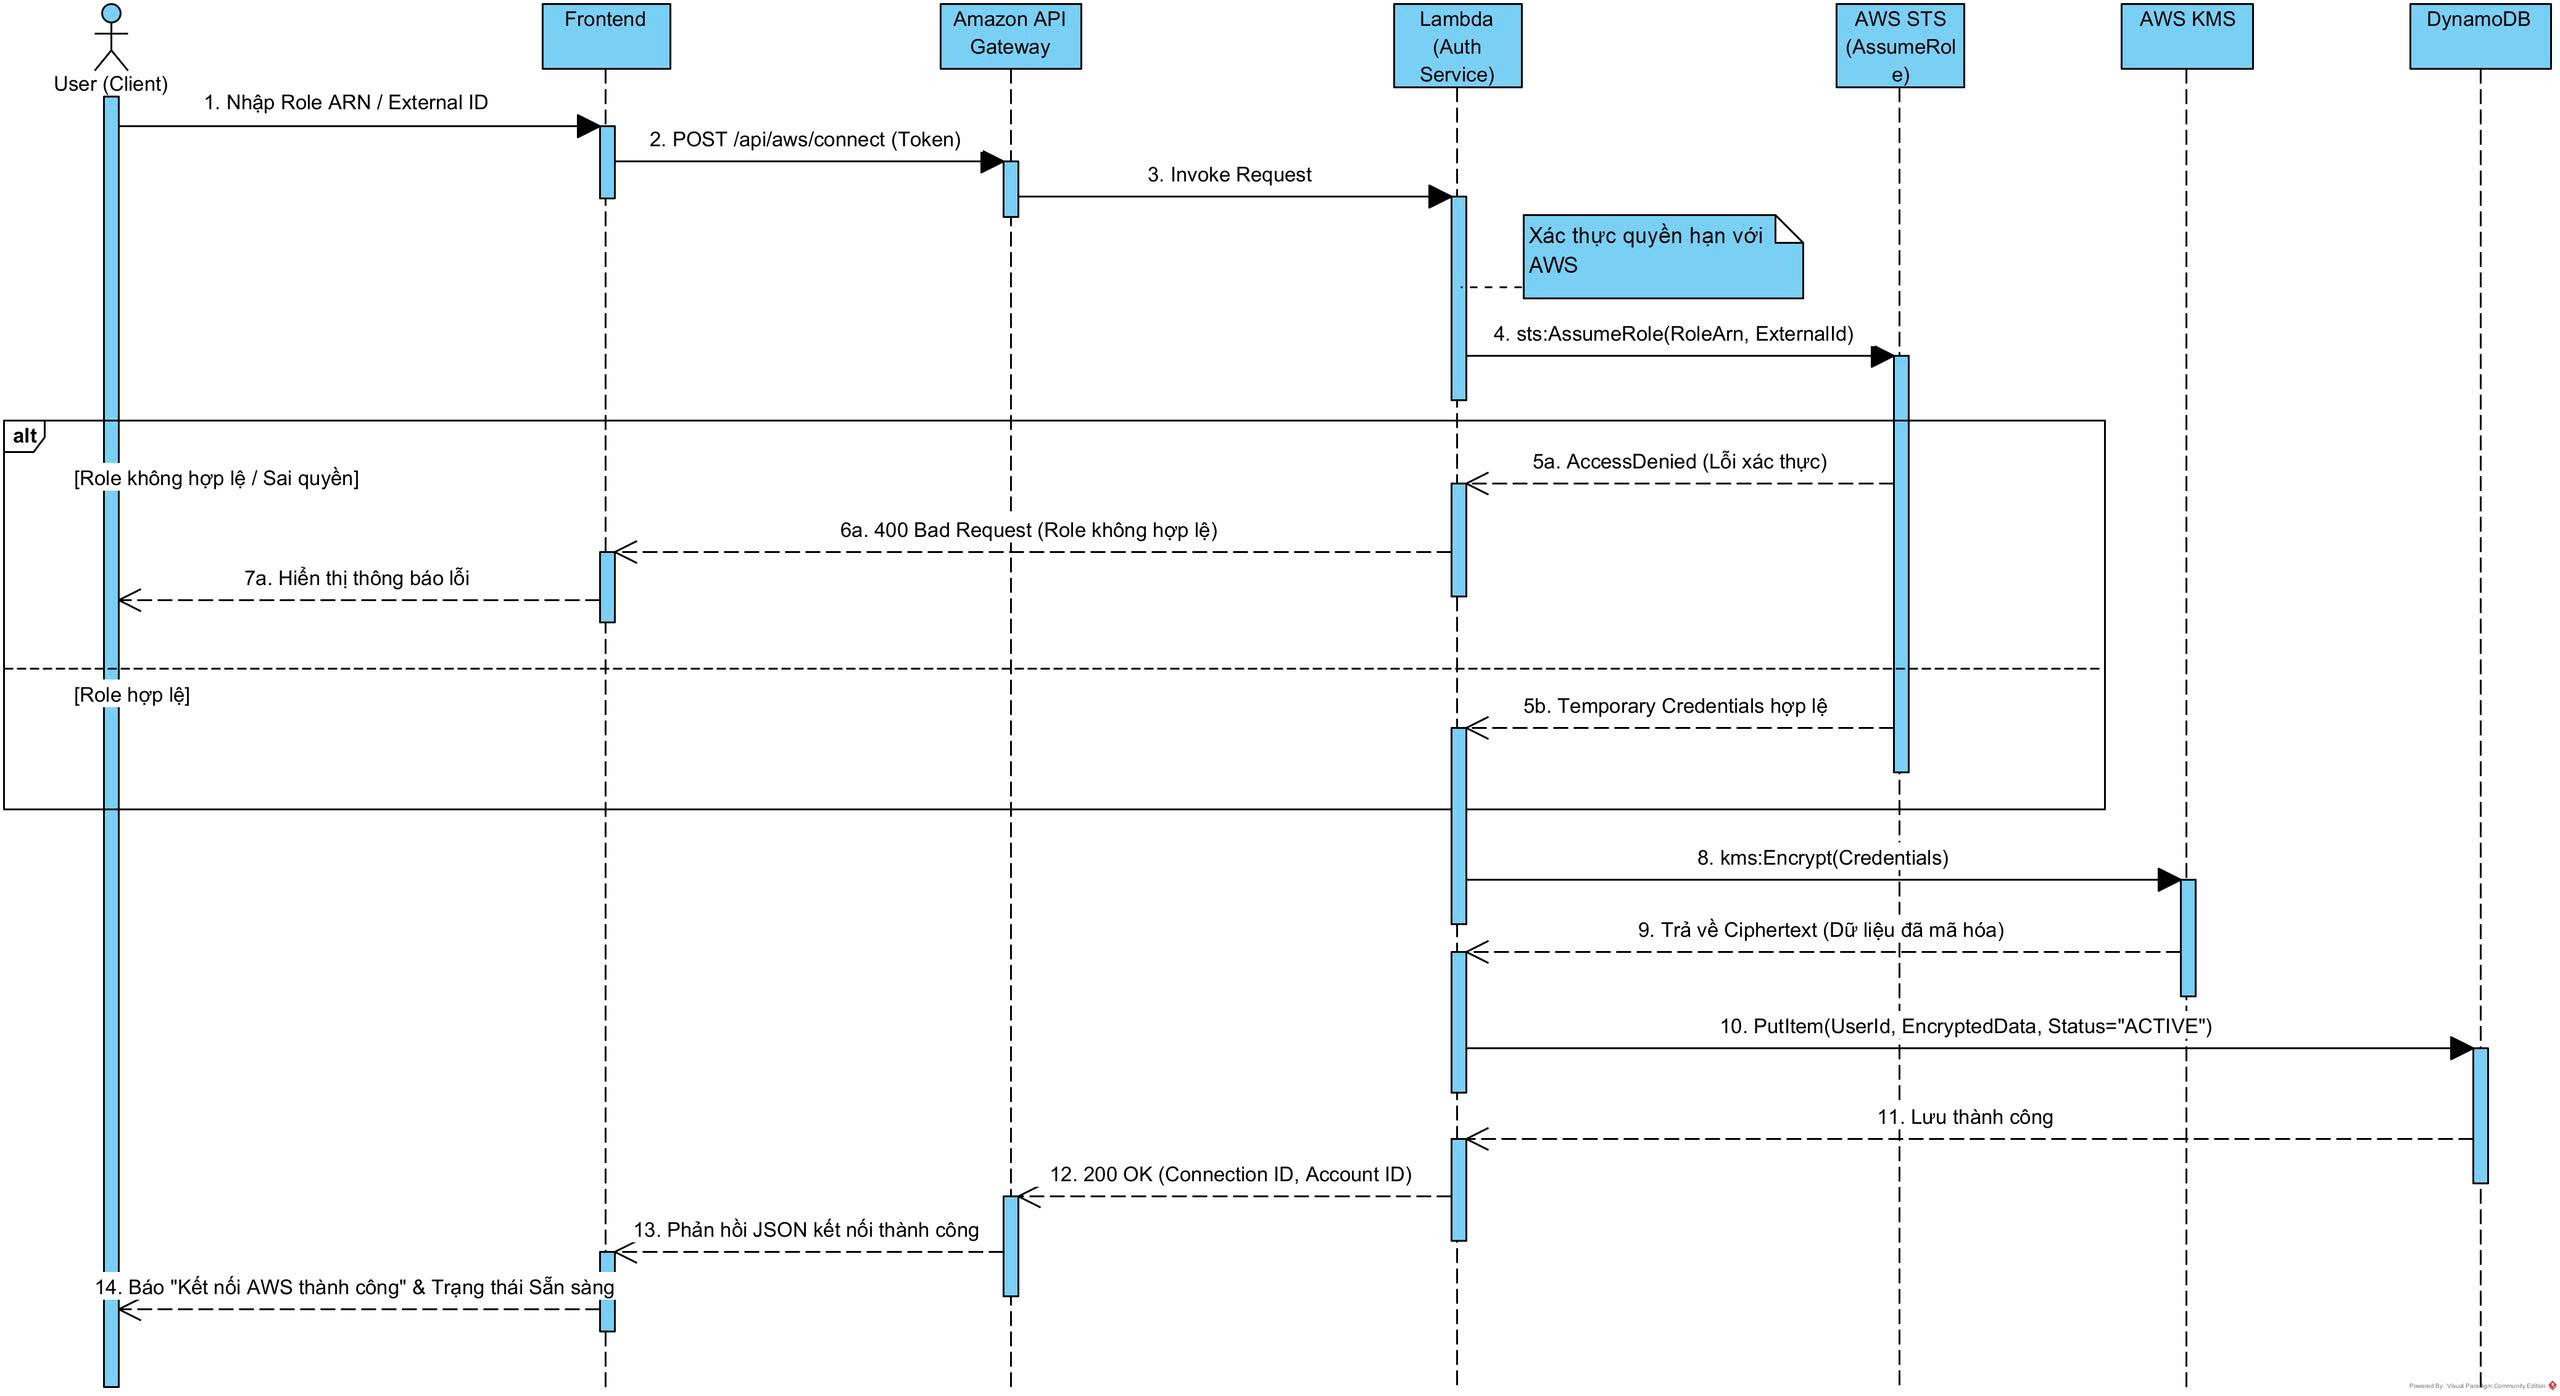
\includegraphics[width=0.88\textwidth]{Image/sequence3.jpg}
  }{
    \fbox{\parbox[c][5cm][c]{0.88\textwidth}{\centering Sơ đồ tuần tự quy trình kết nối tài khoản AWS}}
  }
  \caption{Sơ đồ tuần tự quy trình kết nối và xác thực tài khoản AWS mục tiêu}
  \label{fig:sequence_connect}
  \end{figure}

  \clearpage

  \item \textbf{Phân hệ Quản trị tài nguyên qua Chatbot (ChatOps Resource Management):}
  Là phân hệ xử lý chính, điều phối các thao tác quản trị AWS theo yêu cầu bằng tiếng Việt của người dùng:
  \begin{itemize}
    \item \textit{Xử lý ngôn ngữ và trích xuất tham số (Chatbot Lambda \& Model LLM):} Người dùng nhập yêu cầu qua khung chat. Hàm \textit{Lambda for Chatbot} tiếp nhận chuỗi ký tự, lấy lịch sử hội thoại từ bảng \texttt{SessionState} trên DynamoDB để giữ ngữ cảnh, sau đó gửi câu lệnh kèm định nghĩa công cụ (\textit{Function Calling Schema}) tới mô hình LLM để nhận diện ý định và trích xuất tham số kỹ thuật.
    \item \textit{Kiểm tra an toàn và điều phối thực thi (Dispatcher Lambda \& User Cloud):} Kế hoạch thao tác được chuyển sang hàm \textit{Lambda for dispatcher} để lưu vào bảng \texttt{PendingAction} và yêu cầu người dùng xác nhận. Khi người dùng bấm đồng ý, Dispatcher Lambda gọi AWS STS lấy phiên xác thực tạm thời, dùng thư viện \textit{Boto3 SDK} thực thi thao tác lên tài khoản AWS của người dùng (\textit{User Cloud}) trên 04 dịch vụ: EC2, S3, IAM và Lambda.
    \item \textit{Định dạng dữ liệu và trả kết quả thời gian thực (Formatter Lambda \& AppSync):} Kết quả thực thi từ Dispatcher Lambda được chuyển sang hàm \textit{Lambda for formatter} để định dạng thành bảng hoặc văn bản trực quan, ghi nhật ký vào bảng \texttt{ActionHistory}, đồng thời gọi dịch vụ \textit{AWS AppSync} để gửi kết quả qua WebSocket về giao diện web của người dùng.
  \end{itemize}

  Luồng tương tác của phân hệ này được chia làm hai giai đoạn rõ rệt: Giai đoạn 1 -- Phân tích yêu cầu qua LLM Function Calling và tạo kế hoạch chờ duyệt (\texttt{PendingAction}); Giai đoạn 2 -- Người dùng xác nhận và hệ thống thực thi tác vụ lên hạ tầng AWS qua Boto3 SDK. Chi tiết chu trình tuần tự được thể hiện tại Hình~\ref{fig:sequence_chatops}.

  \begin{figure}[H]
  \centering
  \IfFileExists{Image/sequence1.jpg}{
    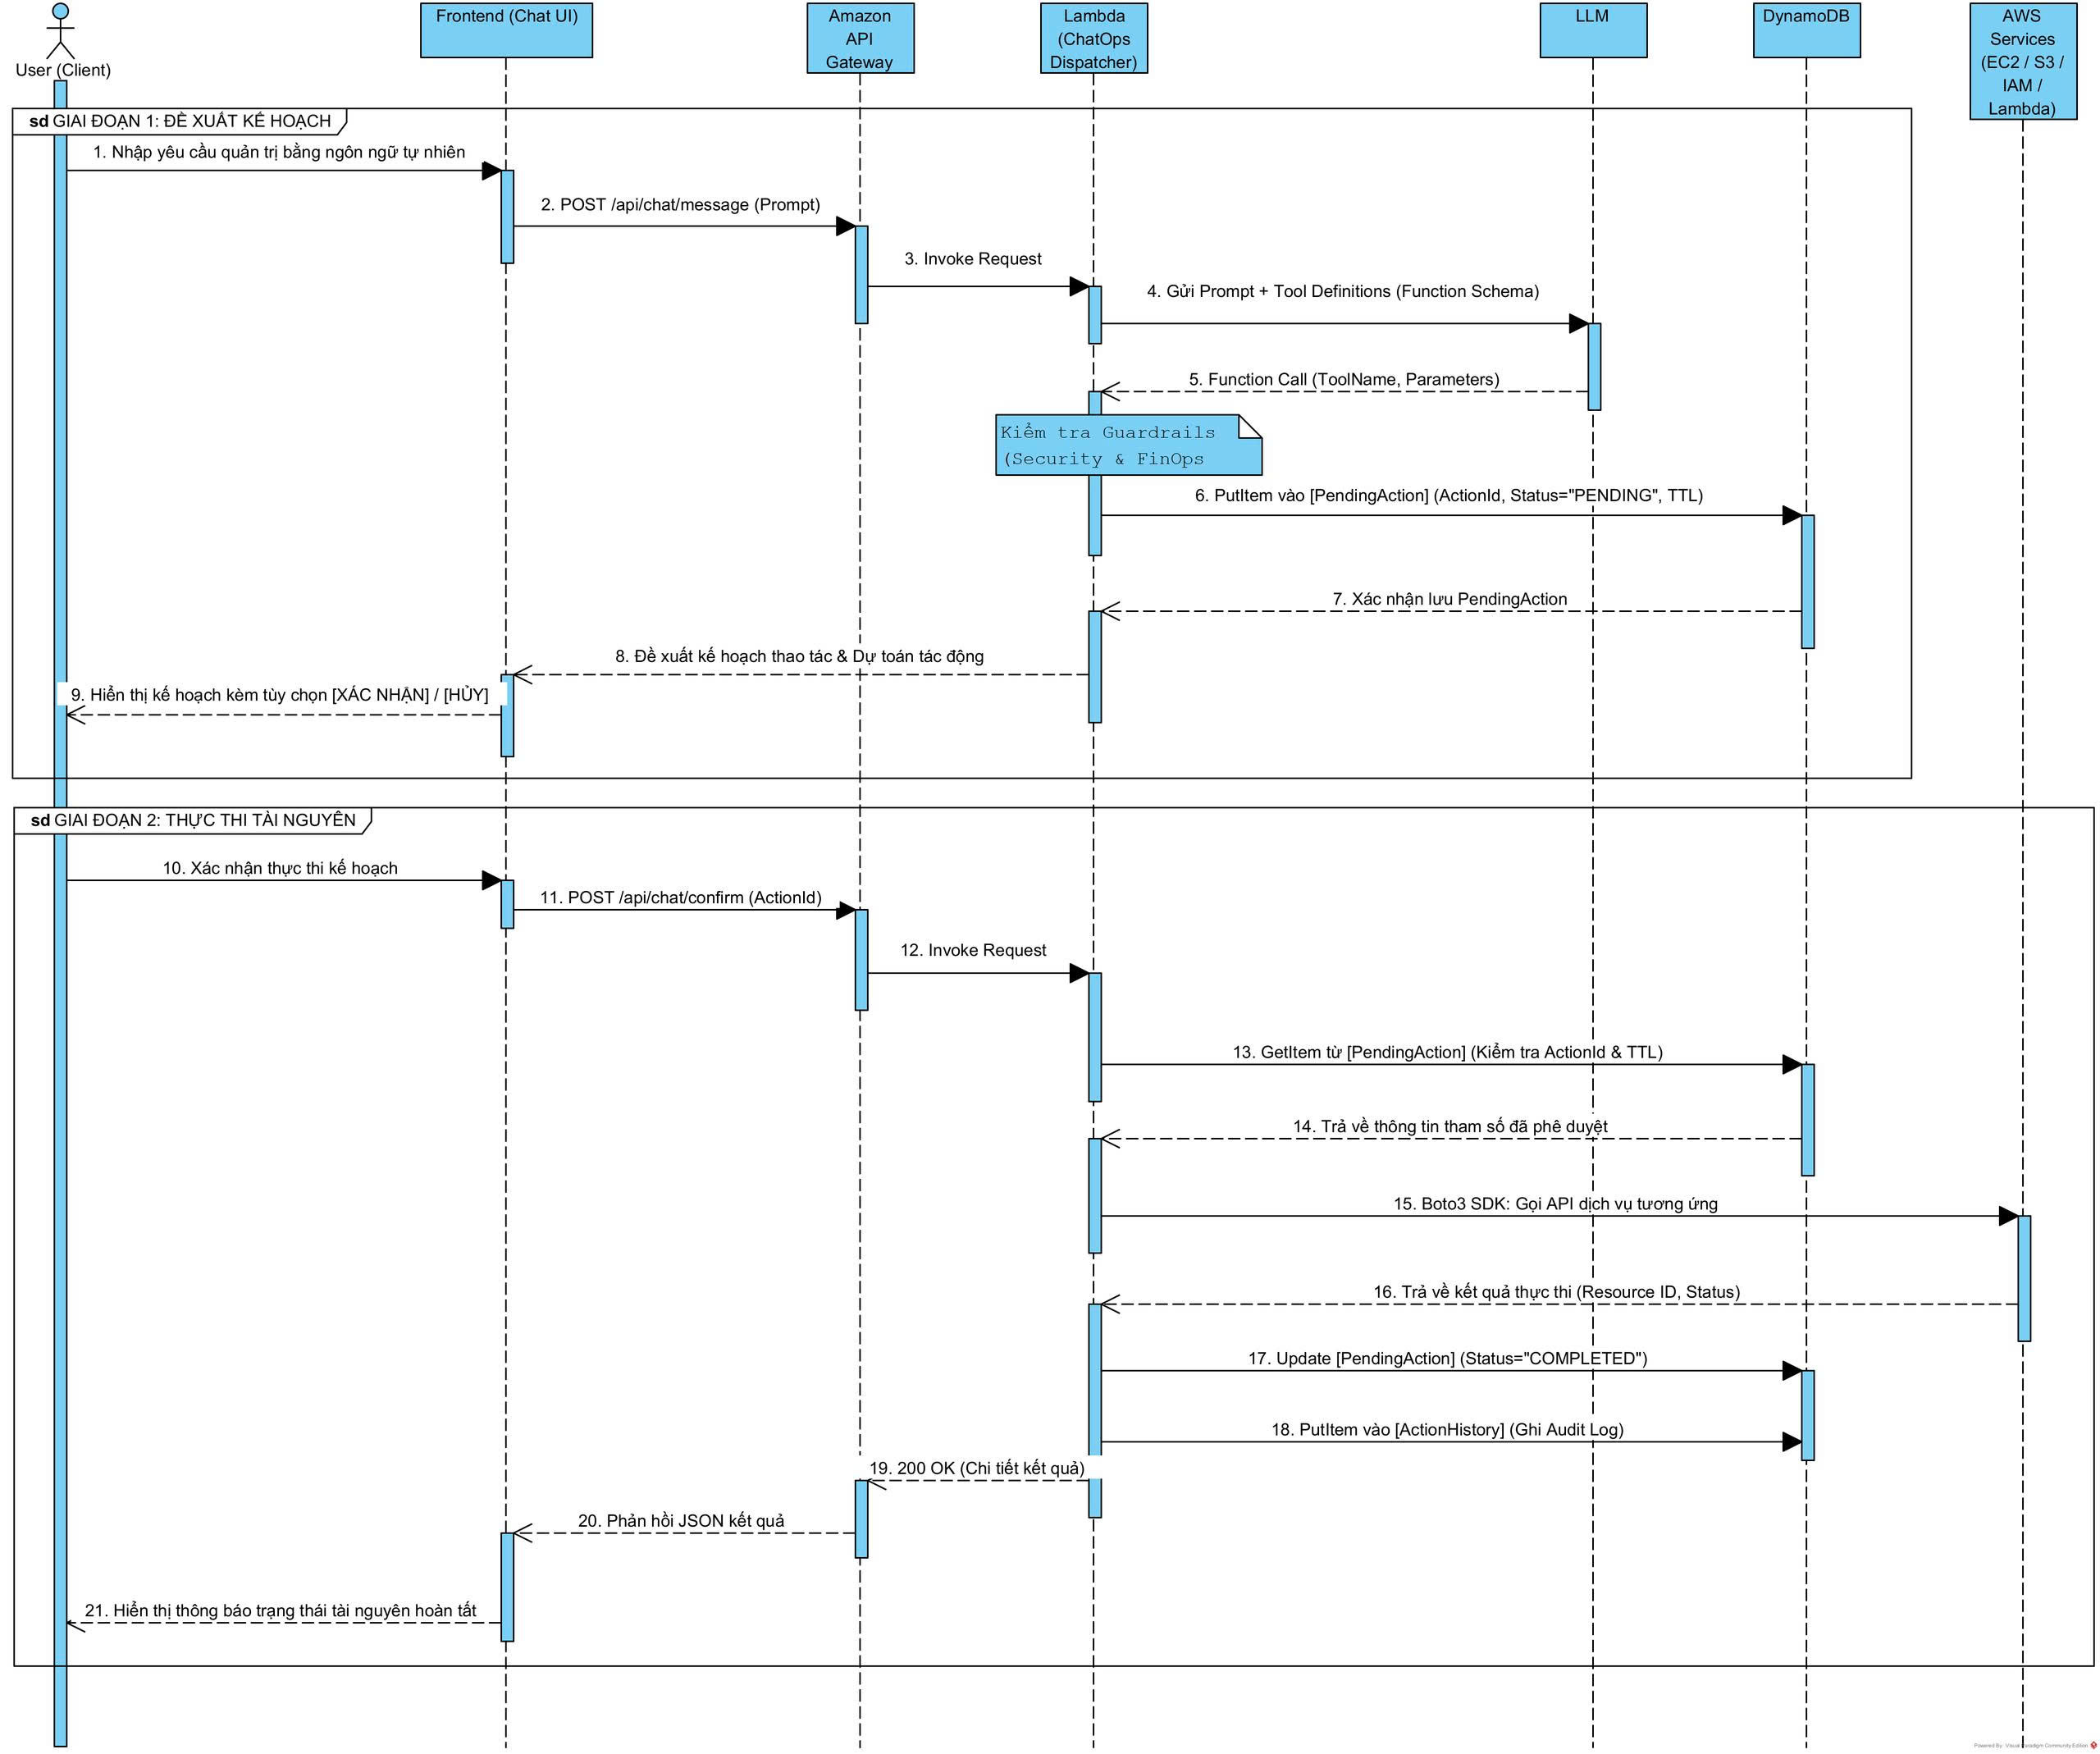
\includegraphics[width=0.68\textwidth]{Image/sequence1.jpg}
  }{
    \fbox{\parbox[c][6.5cm][c]{0.88\textwidth}{\centering Sơ đồ tuần tự quy trình quản trị tài nguyên qua Chatbot}}
  }
  \caption{Sơ đồ tuần tự quy trình điều phối và thực thi tác vụ ChatOps hai giai đoạn}
  \label{fig:sequence_chatops}
  \end{figure}

  \item \textbf{Phân hệ Tra cứu lịch sử thao tác và kiểm toán (History Review \& Audit):}
  Hỗ trợ người dùng theo dõi và kiểm tra lại toàn bộ các thao tác đã thực hiện trên hệ thống:
  \begin{itemize}
    \item \textit{Tiếp nhận yêu cầu tra cứu:} Người dùng gửi yêu cầu xem lịch sử thao tác từ giao diện web hoặc qua câu chat. Yêu cầu được gửi qua API HTTPS tới hàm \textit{Lambda for history review}.
    \item \textit{Truy vấn và hiển thị dữ liệu:} Hàm này đọc dữ liệu từ bảng \texttt{ActionHistory} trên DynamoDB, trích xuất mã hành động, thời gian, tài nguyên đích, người thực hiện và trạng thái kết quả (thành công/thất bại), sau đó hiển thị bảng dữ liệu lên giao diện web.
  \end{itemize}
\end{enumerate}

\clearpage

\subsection{Kiến trúc triển khai của hệ thống}

Hệ thống SatiBot được triển khai dựa trên kiến trúc phi máy chủ (Serverless Architecture) trên nền tảng Amazon Web Services (AWS). Mô hình này giúp tiết kiệm chi phí vận hành (theo hình thức Pay-as-you-go, chỉ tính tiền khi có yêu cầu xử lý), tự động co giãn theo tải (Auto-scaling) và giảm bớt gánh nặng bảo trì máy chủ vật lý.

Bảng~\ref{tab:kientruc} tổng hợp các thành phần và dịch vụ được triển khai trong kiến trúc hệ thống SatiBot.

\begin{table}[H]
\centering
\caption{Các thành phần và dịch vụ trong kiến trúc triển khai hệ thống SatiBot}
\label{tab:kientruc}
\bangfont
\begin{tabularx}{\linewidth}{@{}p{4.8cm}Y@{}}
\toprule
\textbf{Thành phần / Dịch vụ} & \textbf{Vai trò và vị trí trong kiến trúc}\\
\midrule
React & Xây dựng giao diện web ChatOps, hỗ trợ gửi câu lệnh, hiển thị bảng dữ liệu và các nút xác nhận thao tác.\\
Amazon S3 \& Amazon CloudFront & Lưu trữ mã nguồn giao diện tĩnh (HTML, CSS, JS) và phân phối qua CDN CloudFront có chứng chỉ HTTPS.\\
AWS AppSync & Duy trì kết nối WebSocket hai chiều theo chuẩn GraphQL Subscriptions, đẩy kết quả xử lý thời gian thực về trình duyệt.\\
Amazon Cognito & Quản lý thông tin tài khoản, xử lý đăng ký, đăng nhập và cấp phát JWT token để xác thực người dùng tại API Gateway.\\
Amazon API Gateway & Cửa ngõ tiếp nhận các yêu cầu HTTPS REST từ Frontend, kiểm tra tính hợp lệ của JWT token và định tuyến tới các hàm Lambda xử lý tương ứng.\\
AWS Step Functions & Máy trạng thái (State Machine) điều phối tuần tự các bước xử lý nghiệp vụ: Chatbot $\rightarrow$ Dispatcher $\rightarrow$ Formatter.\\
AWS Lambda & Môi trường thực thi code backend Serverless gồm các hàm độc lập: Chatbot, Dispatcher, Formatter, Connector, History và External ID Generator.\\
AWS STS & Cấp phát thông tin xác thực tạm thời (\texttt{sts:AssumeRole}) và kiểm tra quyền của tài khoản khách hàng thông qua cơ chế External ID.\\
Amazon DynamoDB & Cơ sở dữ liệu NoSQL lưu trữ 05 bảng nghiệp vụ: \texttt{Users}, \texttt{AwsConnections}, \texttt{SessionState}, \texttt{PendingAction} và \texttt{ActionHistory}.\\
Python / Boto3 SDK & Thư viện AWS SDK dùng trong các hàm Lambda để gọi API điều khiển tài nguyên AWS trên tài khoản của người dùng.\\
Large Language Model (LLM) & Mô hình ngôn ngữ lớn phân tích nội dung câu chat tiếng Việt, nhận diện ý định và sinh cấu trúc gọi công cụ (\textit{Function Calling}).\\
Amazon CloudWatch & Lưu trữ nhật ký hoạt động (CloudWatch Logs) và theo dõi tình trạng thực thi của các dịch vụ trong hệ thống.\\
\bottomrule
\end{tabularx}
\end{table}

\clearpage

\subsubsection{Sơ đồ kiến trúc triển khai tổng thể và đặc tả giao diện tương tác}

Toàn bộ hệ thống SatiBot được thiết kế theo kiến trúc phi máy chủ (Serverless) trên nền tảng AWS nhằm tối ưu chi phí vận hành và tự động co giãn theo lưu lượng truy cập thực tế. Kiến trúc tổng thể cùng các luồng liên kết giữa các thành phần được thể hiện ở Hình~\ref{fig:so_do_kien_truc}.

\begin{figure}[H]
\centering
\setlength{\intextsep}{6pt}
\IfFileExists{Image/so_do_kien_truc.jpg}{
  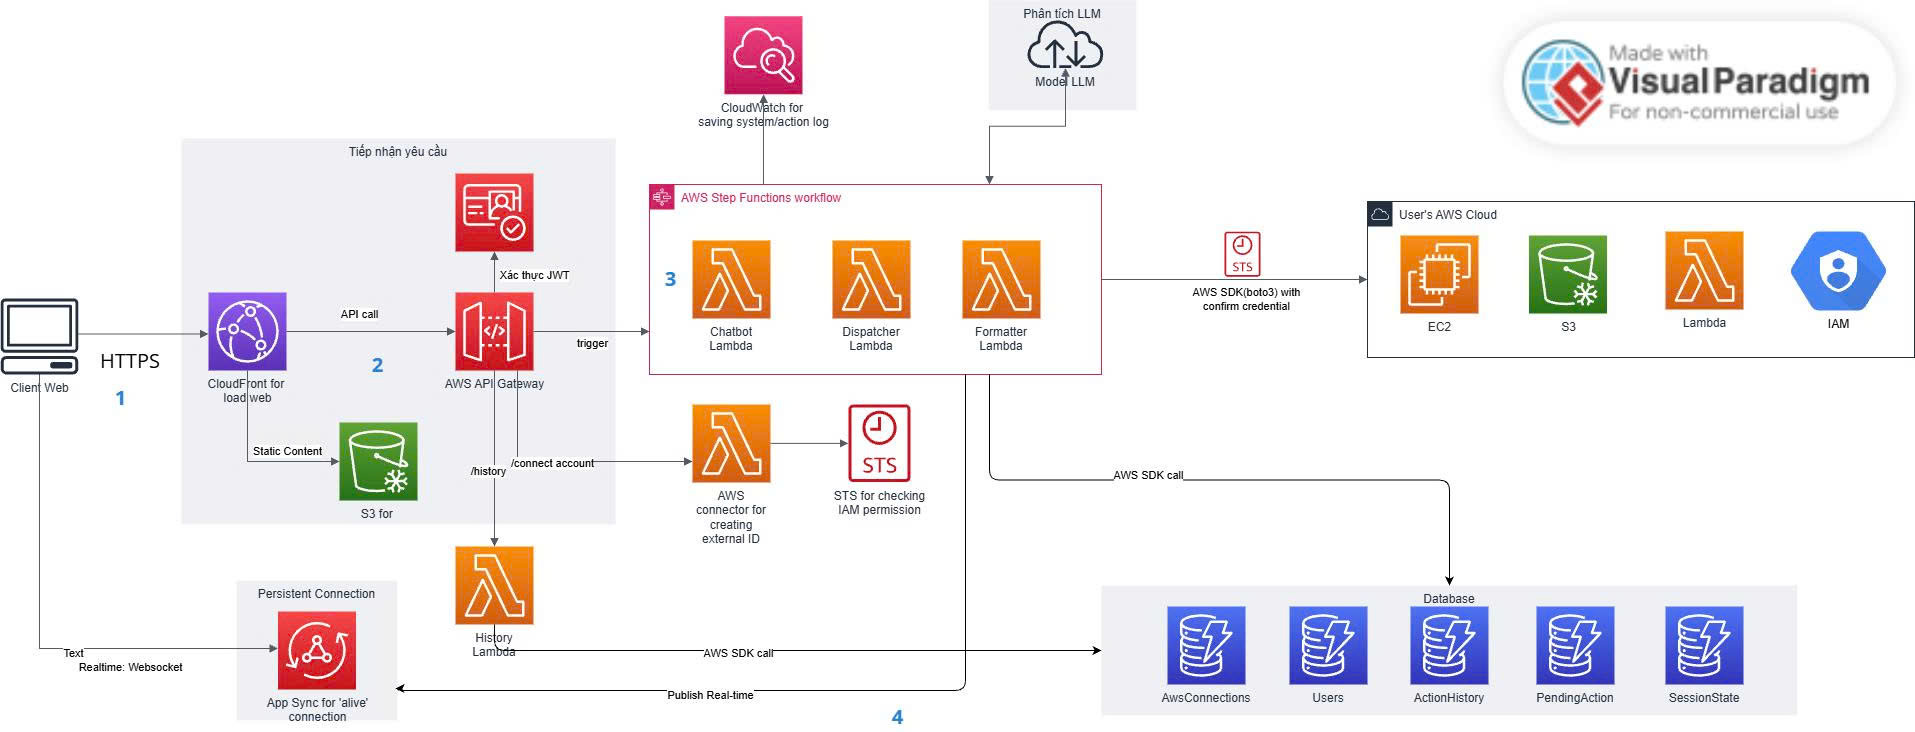
\includegraphics[width=0.62\textwidth]{Image/so_do_kien_truc.jpg}
}{
  \fbox{\parbox[c][6.5cm][c]{0.88\textwidth}{\centering Sơ đồ kiến trúc triển khai tổng thể hệ thống SatiBot}}
}
\caption{Sơ đồ kiến trúc triển khai tổng thể hệ thống SatiBot}
\label{fig:so_do_kien_truc}
\end{figure}

Dựa vào sơ đồ trên, các luồng giao tiếp và giao diện tương tác giữa các thành phần kỹ thuật được tổ chức như sau:

\begin{enumerate}[itemsep=4pt,topsep=2pt]
  \item \textbf{Phân phối Frontend và truyền thông thời gian thực:} 
  Giao diện web (React SPA) được đóng gói và lưu trữ tĩnh trên Amazon S3, phân phối tới người dùng qua CDN Amazon CloudFront bằng giao thức HTTPS (TLS 1.3). Để hiển thị phản hồi từ bot ngay khi tác vụ hoàn thành mà không bắt trình duyệt phải gửi yêu cầu thăm dò liên tục (polling), client duy trì một kết nối WebSocket hai chiều (\texttt{wss://}) tới AWS AppSync thông qua cơ chế GraphQL Subscriptions.

  \item \textbf{Cửa ngõ API và xác thực truy cập (API Gateway \& Cognito):} 
  Mọi yêu cầu nghiệp vụ từ web client (gửi lệnh chat, kết nối tài khoản AWS, xem lịch sử) đều được gửi tới Amazon API Gateway qua giao thức HTTPS RESTful. Tại đây, API Gateway tích hợp Cognito Authorizer để kiểm tra tính hợp lệ của JWT Access Token nằm trong header \texttt{Authorization: Bearer <Token>}. Chỉ các yêu cầu đã xác thực thành công mới được chuyển tiếp vào backend xử lý.

  \item \textbf{Điều phối luồng xử lý ChatOps (Step Functions, Lambda \& LLM):} 
  Luồng xử lý chính được quản lý bởi máy trạng thái AWS Step Functions, kết nối tuần tự 03 hàm Lambda chuyên biệt:
  \begin{itemize}
    \item \textit{Chatbot Lambda:} Nhận payload sự kiện từ API Gateway (theo chuẩn Lambda Proxy Integration), sau đó gọi HTTPS API sang mô hình LLM cùng bộ Tool Schema để bóc tách ý định người dùng và trích xuất tham số kỹ thuật.
    \item \textit{Dispatcher Lambda:} Tiếp nhận kế hoạch hành động, kiểm tra các điều kiện an toàn (Guardrails) và gọi AWS SDK thao tác với hạ tầng đám mây.
    \item \textit{Formatter Lambda:} Nhận kết quả thực thi, chuẩn hóa dữ liệu thành văn bản/bảng biểu trực quan, ghi log kiểm toán và gọi một GraphQL Mutation (HTTPS POST) tới AppSync để bắn kết quả ngược về giao diện người dùng qua kênh WebSocket.
  \end{itemize}

  \item \textbf{Lưu trữ dữ liệu và theo dõi hệ thống (DynamoDB \& CloudWatch):} 
  Hệ thống sử dụng 05 bảng trên Amazon DynamoDB để lưu trữ trạng thái phiên làm việc, thông tin liên kết tài khoản và lịch sử thao tác. Các hàm Lambda đọc/ghi DynamoDB và đẩy log vận hành lên Amazon CloudWatch thông qua thư viện Boto3 trên nền HTTPS. Toàn bộ quyền truy cập được cấp phát riêng rẽ qua IAM Execution Role của từng hàm theo nguyên tắc đặc quyền tối thiểu.

  \item \textbf{Tương tác với hạ tầng AWS của người dùng (User's Cloud):} 
  Để điều khiển tài nguyên (EC2, S3, IAM, Lambda) mà không cần lưu khóa truy cập cố định của khách hàng, Dispatcher Lambda gọi API \texttt{sts:AssumeRole} kèm theo \texttt{RoleArn} và \texttt{ExternalId} tương ứng để nhận về bộ thông tin xác thực tạm thời. Thư viện Boto3 sẽ sử dụng bộ khóa tạm này để tự động ký số các gói tin theo chuẩn AWS Signature Version 4 (SigV4) trước khi gửi tới API Endpoint của AWS.
\end{enumerate}

Thông số kỹ thuật chi tiết của các giao diện tương tác giữa từng cặp dịch vụ được tổng hợp trong Bảng~\ref{tab:inter_service_interfaces}.

\begin{table}[H]
\centering
\caption{Đặc tả giao diện và giao thức tương tác giữa các thành phần trong hệ thống}
\label{tab:inter_service_interfaces}
\begingroup
\renewcommand{\arraystretch}{1.15}
\fontsize{8.5}{11.5}\selectfont
\begin{tabularx}{\linewidth}{@{}>{\raggedright\arraybackslash}p{4.6cm}>{\raggedright\arraybackslash}p{2.4cm}>{\raggedright\arraybackslash}p{3.2cm}Y@{}}
\toprule
\textbf{Giao diện kết nối (Nguồn $\rightarrow$ Đích)} & \textbf{Giao thức / Phương thức} & \textbf{Cơ chế xác thực \& Bảo mật} & \textbf{Định dạng dữ liệu / Payload Contract}\\
\midrule
Web Client $\rightarrow$ S3 / CloudFront & HTTPS (Port 443) & Chứng chỉ TLS 1.3 / ACM & Static HTML/CSS/JS Assets\\
Web Client $\rightarrow$ API Gateway & HTTPS REST (POST, GET) & Cognito JWT Token (Bearer) & JSON Request Body (kèm \texttt{message}, \texttt{connectionId})\\
Web Client $\leftrightarrow$ AWS AppSync & WSS (WebSocket) & Cognito User Pool Auth & GraphQL Subscriptions (JSON Real-time events)\\
API Gateway $\rightarrow$ Step Functions & AWS Service Integration & IAM Resource-based Policy & State Machine Input JSON (Headers, Context, Body)\\
Chatbot Lambda $\leftrightarrow$ Model LLM & HTTPS REST API & API Key / AWS SigV4 & JSON Tool Definition \& Function Arguments\\
Step Functions $\leftrightarrow$ Lambda Tasks & AWS Step Functions SDK & IAM Execution Role & State Machine JSON Context (Task Input/Output)\\
Formatter Lambda $\rightarrow$ AWS AppSync & HTTPS POST & AWS IAM Signing (SigV4) & GraphQL Mutation (\texttt{publishChatMessage})\\
Lambda $\leftrightarrow$ Amazon DynamoDB & AWS SDK (Boto3) & IAM Execution Role & DynamoDB JSON Format (\texttt{PutItem}, \texttt{GetItem}, \texttt{Query})\\
Dispatcher Lambda $\rightarrow$ AWS STS & AWS SDK (HTTPS) & IAM Execution Role & \texttt{sts:AssumeRole} (Payload: \texttt{RoleArn}, \texttt{ExternalId})\\
Dispatcher $\rightarrow$ User's AWS Cloud & HTTPS REST API (Boto3) & \textbf{AWS SigV4} (Temporary Creds) & AWS Service REST API Request / Response JSON\\
\bottomrule
\end{tabularx}
\endgroup
\end{table}

\clearpage

\section{KẾ HOẠCH TRIỂN KHAI DỰ ÁN}

\subsection{Kế hoạch triển khai theo từng giai đoạn (05 tuần)}

Dự án được lên kế hoạch thực hiện trong 05 tuần theo mô hình Agile/Scrum, chia thành 05 Sprint tương ứng với từng tuần phát triển. Mỗi tuần tập trung hoàn thành một nhóm mục tiêu cụ thể, kiểm thử độc lập từng phần trước khi ghép nối hệ thống:

\begin{itemize}
  \item \textbf{Tuần 1 (Sprint 1) -- Chuẩn bị môi trường và kiểm thử PoC độc lập:} Thống nhất quy định làm việc, quy chuẩn viết code chung. Tạo tài khoản AWS chung và IAM User cho từng thành viên. Mỗi thành viên tìm hiểu tài liệu kỹ thuật, viết và kiểm thử độc lập các hàm Python/Boto3 cơ bản cho dịch vụ AWS mình phụ trách (S3, EC2, Lambda, IAM).
  \item \textbf{Tuần 2 (Sprint 2) -- Xây dựng hạ tầng cơ bản và ghép nối Backend:} Dựng khung giao diện web React tĩnh trên S3/CloudFront; cấu hình đăng ký, đăng nhập tài khoản qua Amazon Cognito. Thiết lập API Gateway, viết Lambda Backend tiếp nhận yêu cầu, tạo 05 bảng trên DynamoDB và tích hợp các module Boto3 của 4 thành viên vào Backend.
  \item \textbf{Tuần 3 (Sprint 3) -- Tích hợp AI Chatbot, Step Functions và AppSync:} Tích hợp mô hình ngôn ngữ lớn (LLM), viết prompt và khai báo cấu trúc Function Calling (Tool Schemas). Dựng máy trạng thái Step Functions để điều phối luồng: nhận câu chat $\rightarrow$ Backend gọi LLM trích xuất tham số $\rightarrow$ hiển thị xác nhận $\rightarrow$ xác thực qua STS AssumeRole $\rightarrow$ Boto3 thực thi trên AWS $\rightarrow$ trả kết quả lên giao diện qua kênh WebSocket của AWS AppSync.
  \item \textbf{Tuần 4 (Sprint 4) -- Kiểm thử hệ thống và tối ưu hóa:} Kiểm thử các kịch bản thực tế, bao gồm cả trường hợp chạy thành công và các tình huống thiếu quyền (AccessDenied); cấu hình CloudWatch Logs để theo dõi lỗi tập trung; tối ưu thời gian phản hồi của Lambda và hoàn thiện giao diện chat.
  \item \textbf{Tuần 5 (Sprint 5) -- Nghiệm thu, dọn dẹp tài nguyên và hoàn thiện báo cáo:} Chạy thử toàn bộ các ca sử dụng để nghiệm thu sản phẩm; hoàn thiện báo cáo kỹ thuật, slide thuyết trình; rà soát và xóa các tài nguyên AWS thử nghiệm để tránh phát sinh chi phí.
\end{itemize}

\subsection{Kế hoạch hành động chi tiết theo từng Sprint}

Bảng~\ref{tab:action_plan} liệt kê chi tiết từng đầu việc trong kế hoạch hành động (Action Plan), mối liên hệ với các thành phần trong kiến trúc hệ thống và phân công trách nhiệm cho 04 thành viên tương ứng với 05 tuần (05 Sprint) thực hiện dự án.

\begingroup
\setlength{\tabcolsep}{3.5pt}
\renewcommand{\arraystretch}{1.0}
\fontsize{8.5}{10.8}\selectfont
\begin{longtable}{@{}p{0.6cm}>{\raggedright\arraybackslash}p{3.8cm}>{\raggedright\arraybackslash}p{3.2cm}>{\raggedright\arraybackslash}p{2.6cm}>{\raggedright\arraybackslash}p{4.8cm}@{}}
\caption{Kế hoạch hành động và phân công công việc chi tiết theo từng Sprint}\label{tab:action_plan}\\
\toprule
\textbf{STT} & \textbf{Hạng mục công việc} & \textbf{Thành phần kiến trúc liên quan} & \textbf{Người phụ trách} & \textbf{Kết quả bàn giao}\\
\midrule
\endfirsthead
\caption[]{(Tiếp theo Bảng~\ref{tab:action_plan})}\\
\toprule
\textbf{STT} & \textbf{Hạng mục công việc} & \textbf{Thành phần kiến trúc liên quan} & \textbf{Người phụ trách} & \textbf{Kết quả bàn giao}\\
\midrule
\endhead
\midrule
\multicolumn{5}{r}{\textit{(Còn tiếp sang trang sau...)}}\\
\endfoot
\bottomrule
\endlastfoot
\multicolumn{5}{@{}l}{\textbf{Giai đoạn 1: Tuần 1 -- Thiết lập quy trình, hạ tầng ban đầu và PoC Boto3 độc lập}}\\
1 & Viết và kiểm thử độc lập module Boto3 cho dịch vụ S3 & User's Cloud (Amazon S3) & Phạm Đức Hùng & Module \texttt{s3\_service} (tạo bucket, presign, block public).\\
2 & Thống nhất kịch bản và kiểm thử module Boto3 cho dịch vụ EC2 & User's Cloud (Amazon EC2) & Nguyễn Đức Huy & Module \texttt{ec2\_service} (khởi tạo, bật/tắt, describe).\\
3 & Thống nhất kịch bản và kiểm thử module Boto3 cho Lambda & User's Cloud (AWS Lambda) & Trịnh Thiên Quang & Module \texttt{lambda\_service} (list, invoke, hot config).\\
4 & Thống nhất quy tắc làm việc, tạo tài khoản AWS và module IAM & Toàn bộ kiến trúc, AWS IAM & Cao Anh Minh & Quy chuẩn mã nguồn, AWS Account chung, module \texttt{iam\_service}.\\
\midrule
\multicolumn{5}{@{}l}{\textbf{Giai đoạn 2: Tuần 2 -- Dựng hạ tầng nền tảng Serverless, Giao diện và Tích hợp Backend}}\\
5 & Phát triển khung giao diện React cơ bản trên S3/CloudFront & Frontend (React, S3, CloudFront) & Phạm Đức Hùng & Giao diện Web Chat responsive, CDN CloudFront với HTTPS.\\
6 & Cấu hình luồng đăng nhập và quản lý danh tính qua Cognito & Amazon Cognito, API Gateway & Nguyễn Đức Huy & Luồng Login/Register qua Cognito, JWT Authorizer trên Gateway.\\
7 & Dựng Lambda Backend trung tâm và tích hợp các module Boto3 & AWS Lambda Backend & Trịnh Thiên Quang & Lambda Backend tiếp nhận request và tích hợp các module Boto3.\\
8 & Cấu hình IAM Role cho Backend và thiết kế 05 bảng DynamoDB & AWS IAM, DynamoDB & Cao Anh Minh & IAM Execution Role, 05 bảng DynamoDB cơ sở.\\
\midrule
\multicolumn{5}{@{}l}{\textbf{Giai đoạn 3: Tuần 3 -- Tích hợp AI Chatbot, Step Functions và AppSync}}\\
9 & Định nghĩa Function Calling và Prompt cho dịch vụ S3 & Model LLM, Chatbot Lambda & Phạm Đức Hùng & Bộ Tool Schema cho S3, hỗ trợ kênh WebSocket AppSync.\\
10 & Định nghĩa Function Calling cho EC2 và ghép luồng LLM & Model LLM, Chatbot Lambda & Nguyễn Đức Huy & Bộ Tool Schema cho EC2, hoàn thiện ghép luồng LLM.\\
11 & Tích hợp API LLM, xử lý phản hồi Function Calling tại Backend & Model LLM, Lambda Backend & Trịnh Thiên Quang & Xử lý phản hồi Function Calling và tích hợp LLM vào Backend.\\
12 & Hoàn thiện Prompt IAM, xây dựng Step Functions State Machine & AWS Step Functions, STS & Cao Anh Minh & State Machine điều phối luồng thực thi, xác thực STS.\\
\midrule
\multicolumn{5}{@{}l}{\textbf{Giai đoạn 4: Tuần 4 -- Kiểm thử toàn diện, Phân quyền và Tối ưu hóa}}\\
13 & Kiểm thử hệ thống, tối ưu hóa module S3 & Phân hệ S3, Web Client & Phạm Đức Hùng & Báo cáo kiểm thử S3, tối ưu giao diện truyền tải file.\\
14 & Kiểm thử hệ thống, tối ưu module EC2, dọn dẹp tài nguyên & Phân hệ EC2, CloudWatch & Nguyễn Đức Huy & Báo cáo kiểm thử EC2, kịch bản FinOps cảnh báo máy ảo.\\
15 & Kiểm thử phân quyền, tối ưu hệ thống Backend & Backend Lambda, Step Functions & Trịnh Thiên Quang & Báo cáo kiểm thử phân quyền, tối ưu Cold-start của Lambda.\\
16 & Kiểm thử trường hợp thiếu quyền (AccessDenied), CloudWatch Log & AWS IAM, CloudWatch Logs & Cao Anh Minh & Xử lý lỗi phân quyền, tập trung hóa log trên CloudWatch.\\
\midrule
\multicolumn{5}{@{}l}{\textbf{Giai đoạn 5: Tuần 5 -- Nghiệm thu, Tổng kết dự án và Đóng gói báo cáo}}\\
17 & Hoàn thiện báo cáo phần S3, hỗ trợ làm slide thuyết trình & Báo cáo đề tài & Phạm Đức Hùng & Nội dung báo cáo S3, hoàn thiện slide demo.\\
18 & Tổng hợp kết quả nghiệm thu EC2, chuẩn bị slide demo & Báo cáo đề tài & Nguyễn Đức Huy & Nội dung báo cáo EC2, slide thuyết trình kỹ thuật.\\
19 & Nghiệm thu luồng Lambda, hoàn thiện tài liệu hướng dẫn & Báo cáo đề tài & Trịnh Thiên Quang & Nội dung báo cáo Lambda, tài liệu vận hành.\\
20 & Tổng kết dự án, hoàn thiện báo cáo tổng thể, slide thuyết trình & Báo cáo đề tài & Cao Anh Minh & Bản báo cáo hoàn chỉnh (\texttt{report1.pdf}), slide tổng thể.\\
\end{longtable}
\endgroup

\end{document}
